%%%%%%%%%%%%%%%%%%%%%%%%%%%%%%%%%%%%%%%%%%%%%%%%%%%%%%%%%%%%%%%%%%%%
%% I, the copyright holder of this work, release this work into the
%% public domain. This applies worldwide. In some countries this may
%% not be legally possible; if so: I grant anyone the right to use
%% this work for any purpose, without any conditions, unless such
%% conditions are required by law.
%%%%%%%%%%%%%%%%%%%%%%%%%%%%%%%%%%%%%%%%%%%%%%%%%%%%%%%%%%%%%%%%%%%%

\documentclass[
  digital,     %% The `digital` option enables the default options for the
               %% digital version of a document. Replace with `printed`
               %% to enable the default options for the printed version
               %% of a document.
%%  color,       %% Uncomment these lines (by removing the %% at the
%%               %% beginning) to use color in the printed version of your
%%               %% document
  oneside,     %% The `oneside` option enables one-sided typesetting,
               %% which is preferred if you are only going to submit a
               %% digital version of your thesis. Replace with `twoside`
               %% for double-sided typesetting if you are planning to
               %% also print your thesis. For double-sided typesetting,
               %% use at least 120 g/m² paper to prevent show-through.
  nosansbold,  %% The `nosansbold` option prevents the use of the
               %% sans-serif type face for bold text. Replace with
               %% `sansbold` to use sans-serif type face for bold text.
  nocolorbold, %% The `nocolorbold` option disables the usage of the
               %% blue color for bold text, instead using black. Replace
               %% with `colorbold` to use blue for bold text.
  lof,         %% The `lof` option prints the List of Figures. Replace
               %% with `nolof` to hide the List of Figures.
  lot,         %% The `lot` option prints the List of Tables. Replace
               %% with `nolot` to hide the List of Tables.
]{fithesis4}
%% The following section sets up the locales used in the thesis.
\thesissetup{
    date        = \the\year/\the\month/\the\day,
    university  = mu,
    faculty     = fi,
    type        = bc,
    department  = Department of Machine Learning and Data Processing,
    author      = Dominik Rehák,
    gender      = m,
    advisor     = {RNDr. Vít Novotný, Ph.D.},
    title       = {Generic TeX Writer for the Pandoc Document Converter},
    TeXtitle    = {Generic \TeX{} Writer for the Pandoc Document Converter},
    keywords    = {LaTeX, Lua, Markdown, Pandoc, TeX, text analysis and parsing},
    TeXkeywords = {\LaTeX{}, Lua, Markdown, Pandoc, \TeX{}, text analysis and parsing},
    abstract    = {%
      This is the abstract of my thesis, which can

      span multiple paragraphs.
    },
    thanks      = {%
      These are the acknowledgements for my thesis, which can

      span multiple paragraphs.
    },
    bib         = bibliography.bib,
    %% Remove the following line to use the JVS 2018 faculty logo.
    facultyLogo = fithesis-fi,
}
\usepackage{makeidx}      %% The `makeidx` package contains
\makeindex                %% helper commands for index typesetting.
\usepackage[acronym]{glossaries}          %% The `glossaries` package
\renewcommand*\glspostdescription{\hfill} %% contains helper commands
\loadglsentries{terms-abbrs.tex}          %% for typesetting glossaries
\makenoidxglossaries                      %% and lists of abbreviations.
%% These additional packages are used within the document:
\usepackage{paralist} %% Compact list environments
\usepackage{amsmath}  %% Mathematics
\usepackage{amsthm}
\usepackage{amsfonts}
\usepackage{url}      %% Hyperlinks
\usepackage{markdown} %% Lightweight markup
\usepackage{multicol}
\usepackage{tikz}
\usetikzlibrary{positioning}
\usepackage{listings} %% Source code highlighting
\lstset{
  basicstyle      = \ttfamily,
  identifierstyle = \color{black},
  keywordstyle    = \color{blue},
  keywordstyle    = {[2]\color{cyan}},
  keywordstyle    = {[3]\color{olive}},
  stringstyle     = \color{teal},
  commentstyle    = \itshape\color{magenta},
  breaklines      = true,
}
\usepackage{floatrow} %% Putting captions above tables
\floatsetup[table]{capposition=top}
\usepackage[babel]{csquotes} %% Context-sensitive quotation marks
\usepackage{pdfpages}
\usepackage{graphicx}
\usepackage[export]{adjustbox}

\let\oldlooseness=\looseness
\newcommand{\macro}[1]{\texttt{\textbackslash{}{#1}}}

\begin{document}
%% Uncomment the following lines (by removing the %% at the beginning)
%% and to print out List of Abbreviations and/or Glossary in your
%% document. Titles for these tables can be changed by replacing the
%% titles `Abbreviations` and `Glossary`, respectively.
%% \clearpage
%% \printnoidxglossary[title={Abbreviations}, type=\acronymtype]
%% \printnoidxglossary[title={Glossary}]

\chapter{Introduction}
\emph{Outline the goals of my thesis and the motivations behind them.}

\chapter{State of the art}
\emph{Short outline. Quickly mention discussed utilities.}

\section{Pandoc}
\emph{Pandoc}~\cite{pandoc} is a utility which can convert between dozens of markup and document formats, such as \textsc{html}, docx, various Markdown flavours, \TeX{} formats like \LaTeX{} and Con\TeX{}t or roff for Unix manual pages. It consists of a core Haskell library and a command line tool providing access to this library. % Výstup konverzie je možné ovplyvniť pomocou \emph{filtrov}, čo sú používateľské programy, ktoré upravujú dokument počas konverzie. Pri konverzii do \TeX u má ale autor len obmedzené možnosti, ako ovplyvniť vzhľad výsledných dokumentov.

Internally, the conversion in Pandoc is performed in two phases. First, the input format is converted into a native represenation, also called an \emph{abstract syntax tree} (or \textsc{ast} for short). Then, this \textsc{ast} is converted into the output format. Such a design allows for the input format readers to be written as modules independent of individual output format writers, and vice versa. This also makes it easy to extend the set of Pandoc's supported formats.

It should be noted that a support for a particular format doesn't have to be bidirectional. For example, Pandoc currently provides a Con\TeX{}t writer, but not a Con\TeX{}t reader. Thus, it is possible to implement a reader without a corresponding writer, and vice versa.

The \textsc{ast} itself is exposed via a special format named \texttt{native}, which inputs and outputs the entire \textsc{ast} in Pandoc's internal Haskell representaion. Alternatively, the format \texttt{json} inputs and outputs the \textsc{ast} in the \textsc{json} format. % Keďže existujú rôzne knižnice v~jazyku Lua schopné parsovať formát \textsc{json},\footnote{Knižnica, ktorú naše rozšírenie využíva, je dostupná na \texttt{https://github.com/rxi/json.lua}.} je pre naše rozšírenie Markdownu táto reprezentácia vhodnejšia.

% Je nutné podoktnúť, že Pandoc delí svoje prvky na blokové (block elements) a~neblokové (inline elements). To ovplyvňuje, ktoré prvky sa môžu nachádzať v~potomkoch jednotlivých prvkov a~často korešponduje s~výslednou podobou prvku, napr. implikuje medzery medzi odstavcami, ktoré sú blokovými prvkami. Pri spracovaní \textsc{ast} sa ale týmto rozdelením netreba veľmi zaoberať.

\section{\TeX{}}
\emph{Shortly explain what \TeX{} is and how it differs from \LaTeX{}}.

\subsection{expl3 programming language for \TeX{}}
\emph{expl3 deserves a mention because it greatly simplifies programming in \TeX{}.}

\section{The Markdown package for \TeX{}}
The \emph{Markdown}~\cite{cstug-markdown} \TeX{} package provides the means to embed blocks of text written in the Markdown markup language directly into \TeX{} documents. During the typesetting process, these blocks are parsed and converted into Markdown's own set of intermediate macros, which are then expanded into native \TeX{} macros correspoding to the input.

Markdown's parser originates from a Lua library called \emph{lunamark}~\cite{lunamark}, which is coincidentally also developed by John MacFarlane, the author of Pandoc. lunamark provides a fast conversion of Markdown (its only input format) into other commonly used markup languages, which include \LaTeX{} and Con\TeX{}t. Since Lua\TeX{} is able to run Lua code directly, lunamark's parser was suitable for its use in the Markdown package.

% Rýchlosť konverzie bola jednou z~priorít pri vývoji lunamarku, a~preto konverzia neprebieha v~dvoch fázach (do medziformátu a~z~medziformátu) ako v~prípade Pandocu. Namiesto toho tu dochádza k~priamej komunikácii medzi dvomi modulmi, vstupným (reader) a~výstupným (writer). Výstupný modul implementuje funkcie, ktoré definujú reprezentáciu rôznych prvkov textu vo výstupnom formáte a~vstupný modul počas toho, ako parsuje vstupný dokument, zároveň aj zostavuje výstup s~pomocou funkcií výstupného modulu, ktoré priamo volá.

% Tento princíp bol zachovaný aj v~Markdowne -- s~tým rozdielom, že existujúce výstupné moduly pre podporované formáty boli nahradené jedným, ktorý pre jednotlivé prvky textu generuje makrá \macro{markdownRenderer}\ldots. Tieto makrá je možné predefinovať a~tak upraviť štýl výstupu. Predvolenou hodnotou týchto makier sú makrá \macro{markdownRenderer\textrm{\ldots}Prototype}, ktoré expandujú na natívnu reprezentáciu príslušných prvkov systému \LaTeX{} (viď obr. \ref{fExample page from an \textsc{HTML} document typeset with the proof of concept}ig:markdown-ast} a~\ref{fig:markdown-renderers}).
% \oldlooseness=-1

\emph{Benefits: \LaTeX{} and Con\TeX{}t already supported!}

\subsection{Lunamark writer - a previously explored approach}
Markdown's parser originates from a Lua library called \emph{lunamark}~\cite{lunamark}, which is coincidentally also developed by John MacFarlane, the author of Pandoc. lunamark provides a fast conversion of Markdown (its only input format) into other commonly used markup languages, which include \LaTeX{} and Con\TeX{}t. Since Lua\TeX{} is able to run Lua code directly, lunamark's parser was suitable for its use in the Markdown package.

\emph{Mention the dean's project and what the "original" goal of it was, as well as why the goal eventually shifted (we found a better method).}

\section{Comparison of Pandoc and Markdown}

\emph{Mention differences between the sets of elements.}

(...) Technically, the Markdown packages already provides a plain \TeX{} writer for Markdown. However, using that would only cover the elements of Pandoc \textsc{ast} that are already present in the Markdown format. (...)

\emph{Maybe dump the relevant chapter of the article here!}

\begin{figure}
  \centering
  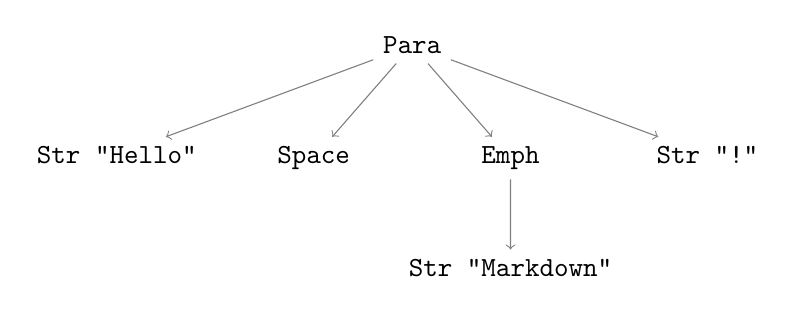
\begin{tikzpicture}[->, anchor=base, baseline, sibling distance=2.5cm]
    \node (pdpara) {\texttt{Para}}
      child { node (pdstrhello) {\texttt{Str "Hello"}} edge from parent[->, gray] }
      child { node (pdspace) {\texttt{Space}} edge from parent[->, gray] }
      child { node (pdemph) {\texttt{Emph}}
        child { node (pdstrmd) {\texttt{Str "Markdown"}} edge from parent[->, gray] }
      edge from parent[->, gray] }
      child { node (exclamation) {\texttt{Str "!"}} edge from parent[->, gray]
    };
  \end{tikzpicture}
  \caption{A graphical Pandoc \textsc{ast} representation for the Markdown input ,,\texttt{Hello *Markdown*!}``}
  \label{fig:pandoc-ast}
\end{figure}

% Prvky Pandocu prevzaté z dokumentácie: \textsf{https://hackage.haskell.org/package/pandoc-types-1.22/docs/Text-Pandoc-Definition.html}

\begin{figure}
  \centering
  \begin{multicols}{3}
    \begin{enumerate}
      \item \texttt{Plain}
      \item \texttt{Para}
      \item \texttt{LineBlock}
      \item \texttt{CodeBlock}
      \item \texttt{RawBlock}
      \item \texttt{BlockQuote}
      \item \texttt{OrderedList}
      \item \texttt{BulletList}
      \item \texttt{DefinitionList}
      \item \texttt{Header}
      \item \texttt{HorizontalRule}
      \item \texttt{Table}
      \item \texttt{Div}
      \item \texttt{Null}
      \item \texttt{Str}
      \item \texttt{Emph}
      \item \texttt{Underline}
      \item \texttt{Strong}
      \item \texttt{Strikeout}
      \item \texttt{Superscript}
      \item \texttt{Subscript}
      \item \texttt{SmallCaps}
      \item \texttt{Quoted}
      \item \texttt{Cite}
      \item \texttt{Code}
      \item \texttt{Space}
      \item \texttt{SoftBreak}
      \item \texttt{LineBreak}
      \item \texttt{Math}
      \item \texttt{RawInline}
      \item \texttt{Link}
      \item \texttt{Image}
      \item \texttt{Note}
      \item \texttt{Span}
    \end{enumerate}
  \end{multicols}
  \vspace*{-1em}
  \caption{Complete list of Pandoc \textsc{ast} elements (as of Pandoc 2.14.2)}
  \label{fig:pandoc-elems}
\end{figure}

\begin{figure}
  \centering
  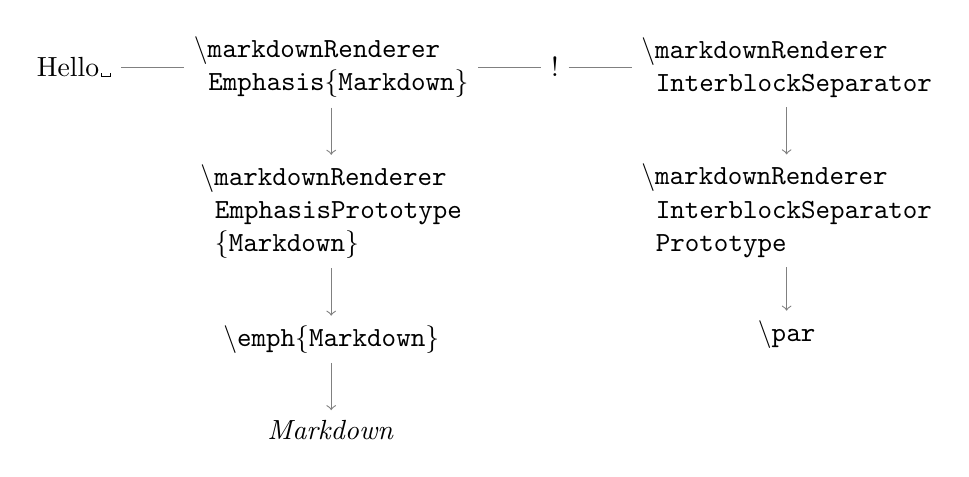
\begin{tikzpicture}[anchor=base, baseline, node distance=0.6cm]
    \node (hello) {Hello\textvisiblespace};
    \node [right=of hello, align=left, xshift=0.2cm] (mdemph) {
      \macro{markdownRenderer} \\
      \texttt{ Emphasis\{Markdown\}}
    } ;
      \node [below=of mdemph, align=left] (mdprotoemph) {
        \macro{markdownRenderer} \\
        \texttt{ EmphasisPrototype} \\
        \texttt{ \{Markdown\}}
      } ;
      \node [below=of mdprotoemph] (texemph) {\macro{emph\{Markdown\}}} ;
      \node [below=of texemph] (emph) {\emph{Markdown}} ;
    \node [right=of mdemph, xshift=0.2cm] (exclamation) {!} ;
    \node [right=of exclamation, align=left, xshift=0.2cm] (mdsep) {
      \macro{markdownRenderer} \\
      \texttt{ InterblockSeparator}
    } ;
      \node [below=of mdsep, align=left] (mdprotosep) {
        \macro{markdownRenderer} \\
        \texttt{ InterblockSeparator} \\
        \texttt{ Prototype}
      } ;
      \node [below=of mdprotosep, yshift=0.14em] (texsep) {\macro{par}} ;

    \path [gray] (hello) edge (mdemph) ;
      \path [gray, ->] (mdemph) edge (mdprotoemph) ;
      \path [gray, ->] (mdprotoemph) edge (texemph) ;
      \path [gray, ->] (texemph) edge (emph) ;
    \path [gray] (mdemph) edge (exclamation) ;
    \path [gray] (exclamation) edge (mdsep) ;
      \path [gray, ->] (mdsep) edge (mdprotosep) ;
      \path [gray, ->] (mdprotosep) edge (texsep) ;
  \end{tikzpicture}
  \caption{Reprezentácia medzimakier a~výstupných makier balíku Markdown pre vstup ,,\texttt{Hello *Markdown*!}``}
  \label{fig:markdown-ast}
\end{figure}

\begin{figure}
  \centering
  \begin{multicols}{2}
    \begin{enumerate}
      \item Tickbox Renderers
      \begin{enumerate}
        \item \texttt{TickedBox}
        \item \texttt{HalfTickedBox}
        \item \texttt{UntickedBox}
      \end{enumerate}
      \item \texttt{InterblockSeparator}
      \item \texttt{LineBreak}
      \item \texttt{Ellipsis}
      \item \texttt{Nbsp}
      \item Special Character Renderers
      \begin{enumerate}
        \item \texttt{Ampersand}
        \item \texttt{Backslash}
        \item \texttt{Circumflex}
        \item \texttt{DollarSign}
        \item \texttt{Hash}
        \item \texttt{LeftBrace}
        \item \texttt{PercentSign}
        \item \texttt{Pipe}
        \item \texttt{RightBrace}
        \item \texttt{Tilde}
        \item \texttt{Underscore}
      \end{enumerate}
      \item \texttt{CodeSpan}
      \item \texttt{Link}
      \item \texttt{Image}
      \item \texttt{ContentBlock}
      \item Bullet List
      \begin{enumerate}
        \item \texttt{UlBegin}
        \item \texttt{UlBeginTight}
        \item \texttt{UlItem}
        \item \texttt{UlItemEnd}
        \item \texttt{UlEnd}
        \item \texttt{UlEndTight}
      \end{enumerate}
      \item Ordered List
      \begin{enumerate}
        \item \texttt{OlBegin}
        \item \texttt{OlBeginTight}
        \item \texttt{OlItem}
        \item \texttt{OlItemEnd}
        \item \texttt{OlItemWithNumber}
        \item \texttt{OlEnd}
        \item \texttt{OlEndTight}
      \end{enumerate}
      \item Definition List
      \begin{enumerate}
        \item \texttt{DlBegin}
        \item \texttt{DlBeginTight}
        \item \texttt{DlItem}
        \item \texttt{DlItemEnd}
        \item \texttt{DlDefinitionBegin}
        \item \texttt{DlDefinitionEnd}
        \item \texttt{DlEnd}
        \item \texttt{DlEndTight}
      \end{enumerate}
      \item Emphasis
      \begin{enumerate}
        \item \texttt{Emphasis}
        \item \texttt{StrongEmphasis}
      \end{enumerate}
      \item Block Quote
      \begin{enumerate}
        \item \texttt{BlockQuoteBegin}
        \item \texttt{BlockQuoteEnd}
      \end{enumerate}
      \item Code Block
      \begin{enumerate}
        \item \texttt{InputVerbatim}
        \item \texttt{InputFencedCode}
      \end{enumerate}
      \item YAML Metadata
      \begin{enumerate}  % nepotrebné?
        \item \texttt{JekyllDataBegin}
        \item \texttt{JekyllDataEnd}
        \item \texttt{JekyllDataMappingBegin}
        \item \texttt{JekyllDataMappingEnd}
        \item \texttt{JekyllDataSequenceBegin}
        \item \texttt{JekyllDataSequenceEnd}
        \item \texttt{JekyllDataBoolean}
        \item \texttt{JekyllDataNumber}
        \item \texttt{JekyllDataString}
        \item \texttt{JekyllDataEmpty}
      \end{enumerate}
      \item Heading
      \begin{enumerate}
        \item \texttt{HeadingOne}
        \item \texttt{HeadingTwo}
        \item \texttt{HeadingThree}
        \item \texttt{HeadingFour}
        \item \texttt{HeadingFive}
        \item \texttt{HeadingSix}
      \end{enumerate}
      \item \texttt{HorizontalRule}
      \item \texttt{Footnote}
      \item \texttt{Cite}
      \item \texttt{TextCite}
      \item \texttt{Table}
      \item \texttt{InlineHtmlComment}
    \end{enumerate}
  \end{multicols}
  \vspace*{-1em}
  \caption{Úplný zoznam výstupných makier balíku Markdown k~verzii 2.11.0}
  \label{fig:markdown-renderers}
\end{figure}

\chapter{Implementation}
\emph{Outline the chapter.}

\section{The custom Pandoc writer itself}
\section{\TeX{} macropackage surrounding the writer}
\subsection{pandoc... macros}
\subsection{pandocInput, shellesc/write18 etc.}
\emph{maybe nějaký veselý historky z natáčení (shellesc, pandocInput, jak pejsek s kočičkou spustili Pandoc z TeXu, codeBlocks v samostatných súboroch + auxdir (haha) etc.)}

\section{Example documents}
\emph{Demonstrate specific example documents and the problems they posed while implementing the writer. \label{fig:html-browsers-typeset} \textbf{Consider if this shouldn't be a separate chapter.}}

% \includepdf[pages={1}]{pandoc-to-markdown/examples/html-browsers.pdf}

\begin{figure}[h]
   \centering
   \begin{tabular}{@{}c@{\hspace{.5cm}}c@{}}
     \includegraphics[
       width=0.6\textwidth,
       page=1,
       frame,
       trim=2cm 2cm 2cm 2cm
     ]{pandoc-to-markdown/examples/html-browsers.pdf}
   \end{tabular}
 \caption{Example page from an \textsc{HTML} document typeset with the proof of concept}
 \label{fig:html-browsers-typeset}
\end{figure}

\chapter{Conclusion}
\section{Future work}
\emph{Mention open issues. Also the Haskell plans, solidification of the macros interface and the relevant ongoing discussion.}

\printbibliography[heading=bibintoc] %% Print the bibliography.

\makeatletter\thesis@blocks@clear\makeatother
\phantomsection %% Print the index and insert it into the
\addcontentsline{toc}{chapter}{\indexname} %% table of contents.
\printindex

\appendix %% Start the appendices.
\chapter{An appendix}
Here you can insert the appendices of your thesis.

\end{document}
